%% 
%% Copyright 2007-2019 Elsevier Ltd
%% 
%% This file is part of the 'Elsarticle Bundle'.
%% ---------------------------------------------
%% 
%% It may be distributed under the conditions of the LaTeX Project Public
%% License, either version 1.2 of this license or (at your option) any
%% later version.  The latest version of this license is in
%%    http://www.latex-project.org/lppl.txt
%% and version 1.2 or later is part of all distributions of LaTeX
%% version 1999/12/01 or later.
%% 
%% The list of all files belonging to the 'Elsarticle Bundle' is
%% given in the file `manifest.txt'.
%% 
%% Template article for Elsevier's document class `elsarticle'
%% with harvard style bibliographic references

% \documentclass[preprint,12pt,authoryear]{elsarticle}

%% Use the option review to obtain double line spacing
\documentclass[authoryear,preprint,review,12pt]{elsarticle}

%% Use the options 1p,twocolumn; 3p; 3p,twocolumn; 5p; or 5p,twocolumn
%% for a journal layout:
%% \documentclass[final,1p,times,authoryear]{elsarticle}
%% \documentclass[final,1p,times,twocolumn,authoryear]{elsarticle}
%% \documentclass[final,3p,times,authoryear]{elsarticle}
%% \documentclass[final,3p,times,twocolumn,authoryear]{elsarticle}
%% \documentclass[final,5p,times,authoryear]{elsarticle}
%% \documentclass[final,5p,times,twocolumn,authoryear]{elsarticle}

%% For including figures, graphicx.sty has been loaded in
%% elsarticle.cls. If you prefer to use the old commands
%% please give \usepackage{epsfig}

%% The amssymb package provides various useful mathematical symbols
\usepackage{amssymb}
%% The amsthm package provides extended theorem environments
%% \usepackage{amsthm}

%% The lineno packages adds line numbers. Start line numbering with
%% \begin{linenumbers}, end it with \end{linenumbers}. Or switch it on
%% for the whole article with \linenumbers.
\usepackage{lineno}
\usepackage[dvipsnames]{xcolor}
\usepackage[capitalize]{cleveref}
\usepackage[inline]{enumitem}
\usepackage{siunitx}
\usepackage{xspace} % required by the \gci command
\usepackage{xparse} % required by the section redefinition
\usepackage{ifthen} % required by the section redefinition

\newcommand{\note}[1]{\emph{\textcolor{red}{#1}}}
\newcommand{\update}[1]{\emph{\textcolor{blue}{#1}}}
\newcommand{\review}[1]{\emph{\textcolor{cyan}{#1}}}
\newcommand{\temp}[1]{\emph{\textcolor{gray}{#1}}}

\let\plainsection\section
\RenewDocumentCommand{\section}{s m o o}{
	\IfBooleanTF{#1}{
		% starred variant, unmodified
		\plainsection*{#2}
	}{
	    \IfNoValueTF{#3}{
	        % standard section
	        \plainsection{#2}
	    }{
	        \IfNoValueTF{#4}{
	            % only the assignee given
	            \plainsection{#2 (#3)}
	        }{
	        	\ifthenelse{
	        		\equal{#4}{todo}
	        	}{
	        		\plainsection{#2 (\textcolor{red}{#3 - TO DO})}
	        	}{}
	            \ifthenelse{
	            	\equal{#4}{wip}
	            }{
	            	\plainsection{#2 (\textcolor{red}{#3 - IN PROGRESS})}
	            }{}  
	        	\ifthenelse{
	        		\equal{#4}{update}
	        	}{
	        		\plainsection{#2 (\textcolor{blue}{#3 - UPDATE})}
	        	}{}
	        	\ifthenelse{
	        		\equal{#4}{review}
	        	}{
	        		\plainsection{#2 (\textcolor{cyan}{#3 - REVIEW})}
	        	}{}
	            \ifthenelse{
	            	\equal{#4}{done}
	            }{
	            	\plainsection{#2 (\textcolor{PineGreen}{#3 - READY})}
	            }{}
	        }
	    }
    }
}

\let\plainsubsection\subsection
\RenewDocumentCommand{\subsection}{s m o o}{
	\IfBooleanTF{#1}{
		% starred variant, unmodified
		\plainsubsection*{#2}
	}{
		\IfNoValueTF{#3}{
		    % standard section
		    \plainsubsection{#2}
		}{
		    \IfNoValueTF{#4}{
		        % only the assignee given
		        \plainsubsection{#2 (#3)}
		    }{
		    	\ifthenelse{
		    		\equal{#4}{todo}
		    	}{
		    		\plainsubsection{#2 (\textcolor{red}{#3 - TO DO})}
		    	}{}
		        \ifthenelse{
		        	\equal{#4}{wip}
		        }{
		        	\plainsubsection{#2 (\textcolor{red}{#3 - IN PROGRESS})}
		        }{}  
		    	\ifthenelse{
		    		\equal{#4}{update}
		    	}{
		    		\plainsubsection{#2 (\textcolor{blue}{#3 - UPDATE})}
		    	}{}
		     	\ifthenelse{
	        		\equal{#4}{review}
	        	}{
	        		\plainsubsection{#2 (\textcolor{cyan}{#3 - REVIEW})}
	        	}{}
		        \ifthenelse{
		        	\equal{#4}{done}
		        }{
		        	\plainsubsection{#2 (\textcolor{PineGreen}{#3 - READY})}
		        }{}
		    }
		}
	}
}

\newcommand{\gci}{\update{AgriMetSupport}\xspace}
% options are: Agriprog, WeatherProg-GCI, AgriSupport, AgriMetSupport, 

\journal{Computers and Electronics in Agriculture}

\bibliographystyle{model2-names}\biboptions{authoryear}

\begin{document}

\begin{frontmatter}

%% Title, authors and addresses

%% use the tnoteref command within \title for footnotes;
%% use the tnotetext command for theassociated footnote;
%% use the fnref command within \author or \address for footnotes;
%% use the fntext command for theassociated footnote;
%% use the corref command within \author for corresponding author footnotes;
%% use the cortext command for theassociated footnote;
%% use the ead command for the email address,
%% and the form \ead[url] for the home page:
%% \title{Title\tnoteref{label1}}
%% \tnotetext[label1]{}
%% \author{Name\corref{cor1}\fnref{label2}}
%% \ead{email address}
%% \ead[url]{home page}
%% \fntext[label2]{}
%% \cortext[cor1]{}
%% \address{Address\fnref{label3}}
%% \fntext[label3]{}

%\title{weatherprog N1 publishing quality-controlled data from heterogeneous stations}
%\title{A cyber-physical infrastructure for agricultural meteorology and planning}
%\title{A platform for agricultural meteorology management \note{and planning (need more in the text)}: \gci }
%\title{Agricultural meteorology management \note{and planning (develop it in the text)}: the \gci platform }
\title{A fully integrated platform for agricultural meteorology management and planning: the \gci at work \note{on data quality control} }

%% use optional labels to link authors explicitly to addresses:
%% \author[label1,label2]{}
%% \address[label1]{}
%% \address[label2]{}

%\author{}
\author[dia]{Giuliano Langella\corref{cor}}
\address[dia]{Department of Agriculture, University of Naples Federico II, Via Università 100, 80055 Portici, NA, Italy}
\cortext[cor]{Corresponding author}
\ead{glangella@unina.it}

\author[deeit]{Raffaele Martino}
\author[deeit]{Massimo Nicolazzo}
\address[deeit]{Department of Electrical Engineering and Information Technology, University of Naples Federico II, Via Claudio 21, 80125 Naples, NA, Italy}

\date{April 2019}

\begin{abstract}
% See the following to write the abstract: https://www.scopus.com/record/display.uri?eid=2-s2.0-85020284965&origin=resultslist&sort=cp-f&src=s&st1=webgis&st2=dss&nlo=&nlr=&nls=&sid=05d242451f19678a21dc297f4479242b&sot=q&sdt=cl&cluster=scosubtype%2c%22ar%22%2ct&sl=30&s=TITLE-ABS-KEY-AUTH%28webgis+dss%29&relpos=3&citeCnt=4&searchTerm=

%[COPIED] The current agrometereological monitoring of the Campania Region is both inadequate for its users and insufficient to support the simulation of pest risk models.
%This work describes a cyber-physical system which has been designed to overcome these limitations, with the objective of
%	\begin{enumerate*}
%		\item automate all the tasks involved in climatic data management, including also the intervention of the human expert when appropriate,
%		\item develop dependable pest risk models and provide the input data they need, and 
%		\item provide real-time agrometereological data presentation.
%	\end{enumerate*}
%	The system is built around an automatic climatic data management engine called WeatherProg, which manages data collection, quality control, data reconstruction, and digital maps production.
%	A proper climatic database has been developed to support the operations of WeatherProg, as well as a Web application for real-time publication of data handled by the software.
%	Pest risk models, fed by point measurements and the digital maps produced by WeatherProg, are going to be prototyped.
%	Furthermore, a new small measurement station has been prototyped, with the aim of being low-cost and easy to relocate, in order to support the characterisation and models parameterisation for different areas.
%	This paper illustrates the current status of the system and discusses future directions.
\end{abstract}

\begin{keyword}
%% keywords here, in the form: keyword \sep keyword

%% PACS codes here, in the form: \PACS code \sep code

%% MSC codes here, in the form: \MSC code \sep code
%% or \MSC[2008] code \sep code (2000 is the default)

\end{keyword}

\end{frontmatter}

\tableofcontents
\linenumbers

%% main text
%\section{}\label{}
\section{NOTES}
\begin{itemize}
    \item Explain exhaustively that \gci is a model GCI that can be easily adapted in every territory with a monitoring net [explain this in discussion and conclusions].
    \item highlight the multi-level modularity, at level of the GCI (also thanks to the docker ecosystem), at level of WeatherProg i.e. (de-)activating modules as required (ftp, decode, qcheck, infill, tscaleconv, pointprevmod, spatinf, gridprevmod), at the physical level i.e. 1 monitoring network (RAR), two monitoring nets (RAR + Prot.Civ.), additional LCN net/station
\end{itemize}






\section{Introduction}[Giuliano][done]

%journal: Computers and Electronics in Agriculture
% https://www.journals.elsevier.com/computers-and-electronics-in-agriculture

% ==== Big Picture ====
%Include the big picture: The Earth Critical Zone requires that models such as SPA and pest models have quality checked data.
%\begin{itemize} 
%    \item Problem statement
%    \item Related work
%    \item Objectives
%\end{itemize}

% ==== Earth Critical Zone ====
%It is a living, breathing, constantly evolving boundary layer where rock, soil, water, air, and living organisms interact. These complex interactions regulate the natural habitat and determine the availability of life-sustaining resources, including our food production and water quality.
%The Critical Zone (CZ) is the support system for all terrestrial ecosystems, extending from unweathered rock to the top of any vegetation canopy. In the CZ, physical, biological, geological and hydrological processes interact at multiple temporal and spatial scales.
%Earth's critical zone is the “heterogeneous, near surface environment in which complex interactions involving rock, soil, water, air, and living organisms regulate the natural habitat and determine the availability of life-sustaining resources”
Climate controls the Earth's Critical Zone (ECZ) in combination with other physical, biological and geological processes.
The ECZ is a heterogeneous system extending from the top of the vegetation canopy to the bottom of unweathered rocks, regulates the availability of resources and modulates the production of ecosystem services such as the filtration and quality of water, and the production of food and fibre.

% ==== Agricultural Meteorology ====
% LINKS:
%   https://books.google.it/books?id=vdFBDwAAQBAJ&pg=PA22&lpg=PA22&dq=importance+of+agrometeo+measurements&source=bl&ots=CmcFAArYyq&sig=ACfU3U1TMqCpGqAv7VZjSz1M_IgPKv1--w&hl=it&sa=X&ved=2ahUKEwjPs_Tdg_vgAhXQ4KQKHYM3B4AQ6AEwAHoECAkQAQ#v=onepage&q=importance%20of%20agrometeo%20measurements&f=false
%   http://www.agrometeorology.org/files-folder/repository/gamp1.pdf
%   https://en.wikibooks.org/wiki/Introductory_Agrometeorology/Introduction
%   http://www.agrilearner.com/agrometeorology-needs-scope/
%   http://www.agriinfo.in/default.aspx?page=topic&superid=1&topicid=377

%Weather: Physical state of the atmosphere at a given place and given time. Eg. Cloudy day
%Climate: Long term regime of atmospheric variables of a given place or area. Eg. Cold season
%and considered as basic input or resources in agricultural planning, every plant process related with growth development and yield of a crop is affected by weather.

Weather and climate are the most important dynamic components of the ECZ determining the physical condition in which animals and plants are grown.
Agricultural meteorology is concerned with the monitoring of weather and the characterisation of the meteorological, hydrological and pedological factors that have a direct effect on agriculture and the production of crop and livestocks.
% http://www.agriinfo.in/default.aspx?page=topic&superid=1&topicid=377
Agricultural meteorology is deemed important considering the large amount of ground stations available worldwide to monitor the behaviour of weather elements, notwithstanding, for instance, the huge amounts of air-borne proxy products coming from massive satellite monitoring.
Indeed, amongst others, it helps: % \note{(search one or more REFs for each item)}: 
    \begin{enumerate*}
        \item understanding the realisation of several crop parameters such as the growing season and the harvesting time;  %\citep[e.g.]{Hoogenboom:agrometeo-swat:2000};
        \item managing crops by means of various farm operations such as fertilisers application and irrigation scheduling;
        \item assessing the suitability of specific crops in space (by means of agroclimatic zoning) and time (e.g. according to climate change);
        \item crop and livestock monitoring and modelling;
        \item understanding the spatial distribution of soil types and properties since climate is one of the soil forming factors recognized in the CLORPT \citep{jenny:clorpt:1941} and SCORPAN \citep{McBratney:scorpan:2003} models;
        \item forecasting plant pests and diseases.
    \end{enumerate*}

There is an increasing demand for the production, in digital format, of weather and climatic data of good quality within the earth critical zone both 
    for practical applications (e.g. the need to know climatic patterns in a farm to improve the management),
    and
    for research and development, in particular to simulate the soil-plant-atmosphere system \citep{Hoogenboom:agrometeo-swat:2000,Jones:swat:2003,Langella:rainann:2010,Seneviratne:swat:2010} and the risk of pests \citep{Orlandini:plasmopara:2008,Rossi:vitenet:2014,Terribile:dssvitis:2017}.
The demand is particularly burdensome considering the requirement to handle climatic data both at finer temporal scale and in a continuous spatial domain.
It means that daily (e.g. in the soil hydrological modelling) or even hourly records (e.g. in the phytopathologic risk modelling) measured at point gauges sparsely located in a territory must be transformed in three dimensional climatic data cubes (Longitude, Latitude, Time) by means of statistically sound geospatial procedures.
% (there is a gap between the major of scientific modelling approaches that requires digital climate maps and the gauged measurements).
There exist few approaches implementing and deploying automatic spatial inference engines of this kind based on point climatic data at the daily or even at the hourly time step.
One example working in USA using already checked daily data, is given by the expert-based model called PRISM developed by  \cite{Daly08_PRISM_USA}. %\note{(search for other REFs? may be sufficient!)}

% ==== Aim ====
%Support systems to agrometeorological practices and services comprise data (so quantification), research, training/education/extension and policy environments. Especially in industrialized countries mathematical models are increasingly used in operational agricultural meteorology, in conjunction with Geographic Information Systems (GISs) to provide inputs to Decision Support Systems (DSSs).
Especially in more developed countries, mathematical models are increasingly used in agriculture in conjunction with Geographic Information Systems (GISs), also via web in the form of WebGIS, to provide inputs to Decision Support Systems (DSSs), possibly via web in the form of Web Based geoSpatial Decision Support Systems (WB-SDSS).
Examples of WB-SDSS can be found 
for heavy metal pollution management in soils \citep{Wang:wbsdss:2005}, 
for livestock manure management \citep{Acutis:wbsdss:2014}, 
for locust prevention and control \citep{Yao:wbsdss:2017}, 
for optimized crop irrigation \citep{Giusti:wbsdss:2015}, 
for land management and soil conservation \citep{Terribile:soilconsweb:2015}, 
and so forth.
There exist a huge production of DSS tools on quite every issue related to the agricultural and forestry systems.
%\note{what is missing? a GCI on agrometerological data to facilitate the assembly of tools to support decision process in issues related to agriculture and forestry.  }
\note{[ENHANCE]} To authors' knowledge, there is a complete gap in literature about Geospatial Cyber-Infrastructure (GCI) fully dedicated to agriculture meteorology, both to implement a stand-alone agrometeorological platform and to facilitate the assembly of tools to support the decision process in issues related to agriculture and forestry. \note{[we might add a note including the SCOPUS search results]}
% To authors' knowledge there is any work in literature dealing with GCI
% SCOPUS = "geospatial cyber infrastructure agrometeorology" ==> 0 results
% SCOPUS = "cyber infrastructure agrometeorology" ==> 0 results
% SCOPUS = "cyberinfrastructure meteorology" ==> 13 results, but not pertinent
% SCOPUS = "geospatial agrometeorology decision support" ==> 0 results

In this paper a strongly modular GCI, called \gci
is proposed as a general technological framework being a WB-SDSS, that can be fully tailored to the specific needs of an existent agrometeorological network (e.g. those managed by local government agencies).
The proposed GCI is based on a software component, namely WeatherProg \citep{langella:weatherprog2014,langella:weatherprog2016}, which represents the main engine of the information technology system and has the potential of being the basic engine of whatever geospatial-based service in agriculture, in which both the weather and the climatic information is of paramount importance.
WeatherProg has the key advantage of implementing all the tasks from gathering the raw measurements coming from the agrometeorological sensors till the delivery of digital climatic maps at different time steps (e.g. hourly, daily, and so forth).

Together with the presentation of the general template WB-SDSS, the results of applying the \gci GCI to a specific case study, that is in Campania Region (South of italy), is shown with the specific focus of producing data of good quality.
The task consists in tuning a fully automatic or assisted procedure to quality check the measurements at the gauged points.
This is of particular relevance due to limitations and constraints (showed in \cref{sec:qcheck}) of the Campania Region agrometeorological network.

\review{The presentation of the work is organised in the paper following a hierarchical structure, starting from the most general part to more particular one. In section \ref{sec:gci} the overall geospatial cyberinfrastructure implementing the decision support system is presented. In section \ref{sec:weatherprog} the core engine processing the agrometerological data is showed with emphasis on main modules and their role in the infrastructure. Section \ref{sec:qcheck} shows the specific tasks of the data quality check, highlighting the operations required to produce data of good quality to be used in cascade in other applications. An application of the \gci GCI to a real case is presented in section \ref{sec:casestudy} (in Campania Region, South of Italy),  with particular focus on ease of implementation and customization, and high flexibility of the whole platform and its components. }

\section{The cyber-physical infrastructure \gci}[Giuliano, Raffaele][review] \label{sec:gci}
%Central to the design of an effective automated data-processing system is the database. The telecommunications subsystem database must hold:
%(a) Bulletins of incoming messages;
%(b) Locally generated observations;
%(c) Products for national dissemination;
%(d) Bulletins of locally generated observations for transmission on the GTS.
%The applications subsystem database must hold:
%(a) Reports derived from decoded bulletins;
%(b) Fields derived from decoded bulletins;
%(c) Products prepared through the processing of reports and fields.
%If possible, the database residing in each computer should be controlled by the same database
%management system (DBMS), which should be relatively simple so as to minimize computing overheads and facil- itate the speed of response of the overall data-processing system.

\gci is designed to be a comprehensive framework for agrometereological monitoring and data management.
\note{[ENHANCE]} It can be effectively used for a wide range of purposes, from simple agrometeorogical monitoring to digital climatic maps production and agricultual and forestry modeling and application, including predictive pest modeling.
Clearly, different real-world applications have different requirements, which can be all accomodated by \gci thanks to its strongly modular architecture.
Components can be added or removed to a specific instance of \gci effortlessly without affecting other parts of the system, as well as modules of the core engine, WeatherProg, which can be selectively enabled or disabled.
This way, end users (e.g. local government agencies) actually derive their own tailored instances from the general model of \gci.

The high-level complete architecture is illustrated in \cref{cyberPhysicalSystemFig}.
At the topmost level, \gci is constituted by central components, responsible for storage and processing of data (e.g. WeatherProg), and peripheral components, in charge of collecting data from the environment (i.e. sensors in the network) or those delivering web services (e.g. agrometeorological data consulting).

\begin{figure}
	\centering
	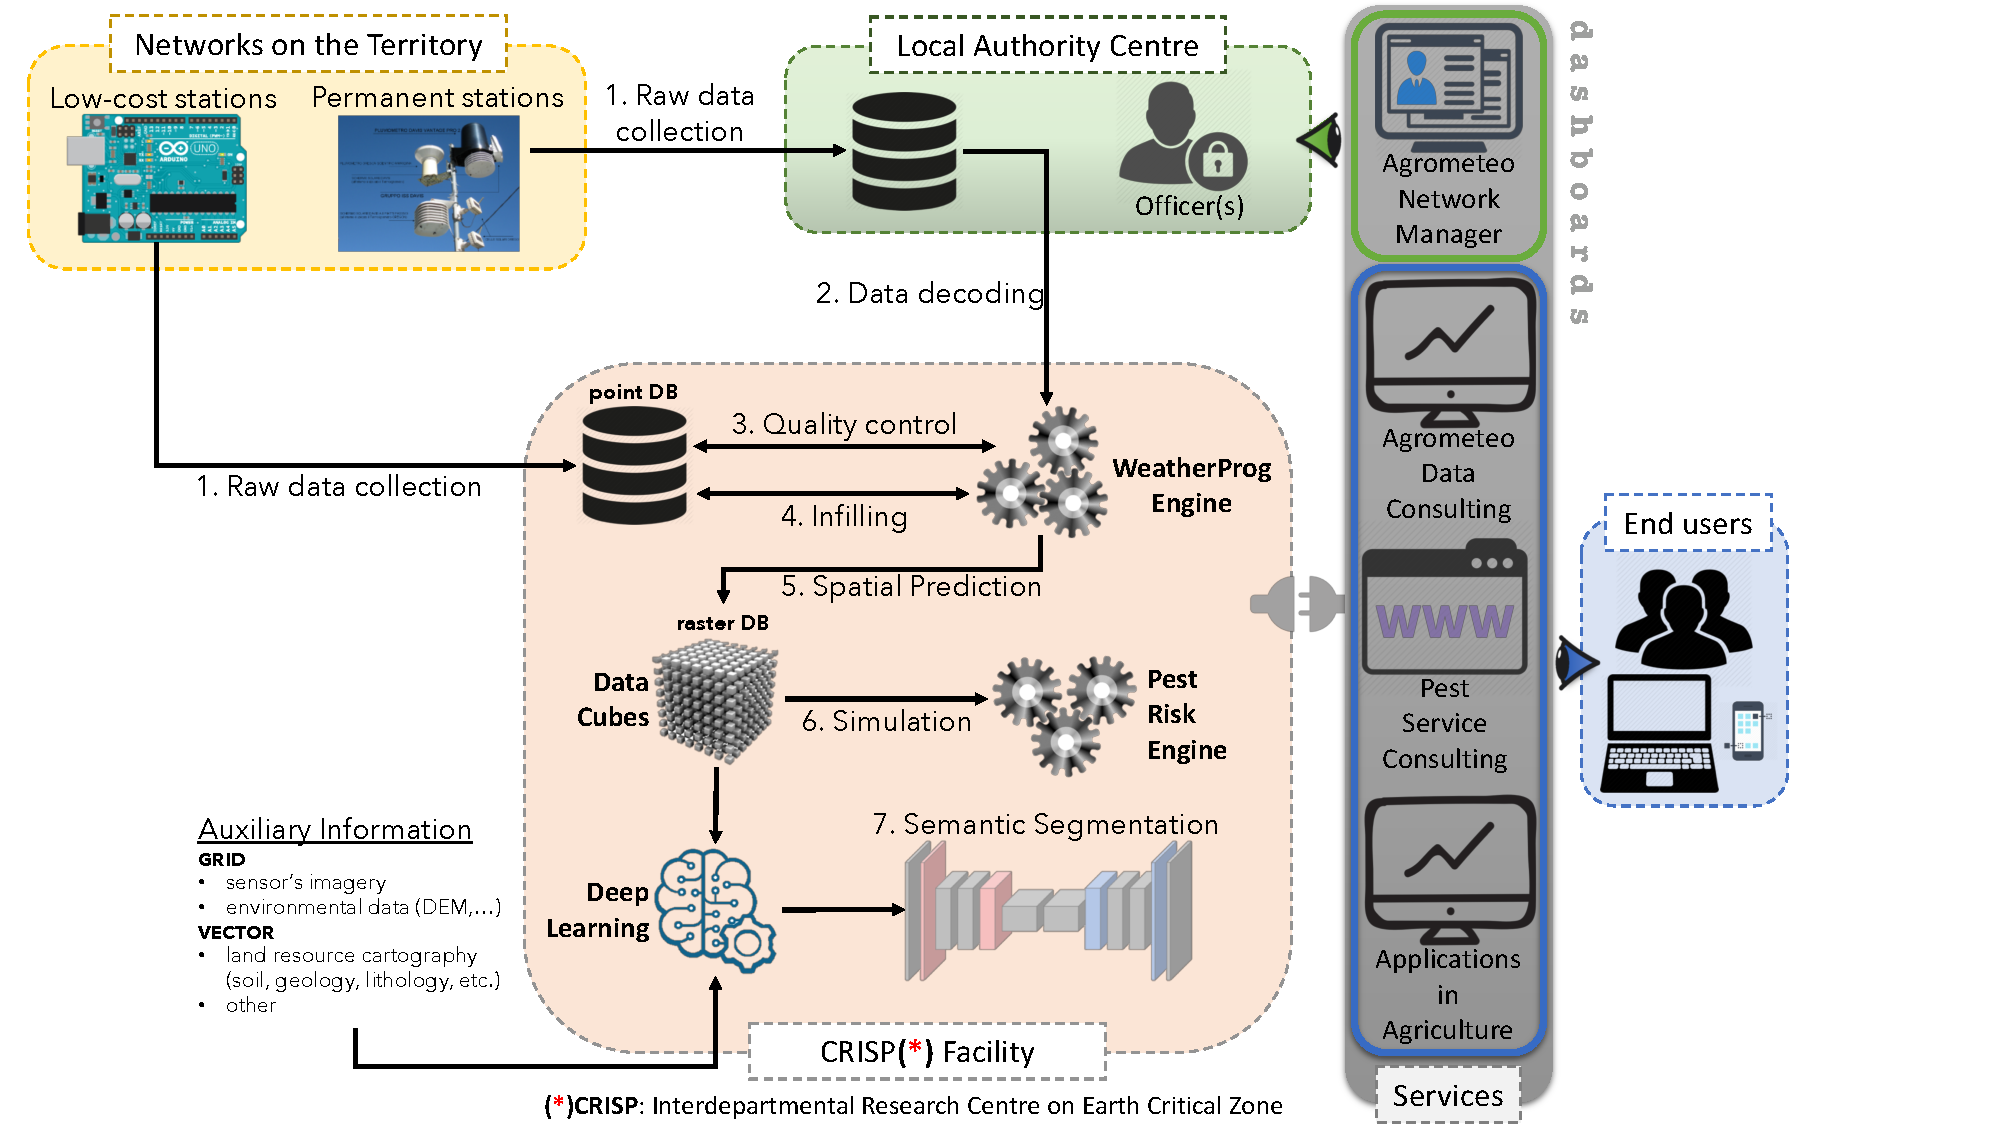
\includegraphics[scale=.5]{figures/fullSystem_GCI.pdf}
	\caption{High level architecture of the \gci cyber-physical system. \note{The deep learning block is speculative and is not part of the GCI yet.}}
	\label{cyberPhysicalSystemFig}
\end{figure}

Peripheral components are the actual monitoring networks.
In fact, \gci is capable of handling and integrating data coming from multiple heterogeneous networks of stations, possibly under the responsibility of different agencies working in the same territory.
Each network can include different kinds of station, and each network can submit data to \gci in different formats, since the decoding module of WeatherProg can be configured to accommodate such differences.
The opportunity to integrate networks is of paramount importance to systematically optimise the joint management of public and/or private monitoring infrastructures with significant beneficial impact on costs savings and services enhancements.
%and reciprocal impact both on the different agencies sharing their data and on farmers and end users who can enjoy more accurate data and less uncertain services.

\gci can also be employed in contexts where there is an insufficient monitoring network coverage of the territory.
In fact, it comes with its own monitoring network, characterised by low-cost stations which are particularly suitable for temporary deployments and for tuning the parameters of the various models included in the GCI.  \note{[MINI + FULL PAPER: Martino, Langella, Nicolazzo 2019]}.
It must be stressed that the low-cost monitoring network is entirely optional, being a component like the others that can be simply removed if there is already excellent coverage of the territory, therefore not preventing the use of \gci in such scenarios. \note{[add installation of low cost station by farmers]}

The main central components are the WeatherProg core engine, and the data bases. Two main data bases are employed by \gci.
The first is a relational data base used to store the climatic data of the station  \review{in a WMO-compliant fashion}.
The latter  is a raster data base capable of handling the digital climatic maps which can be produced as tiles by the WeatherProg engine.
An open source array database is used to stitch together the 2D maps or tiles calculated over time on the different agroclimatic variables to produce multi-dimensional arrays or data cubes, which are  characterised by three (X, Y, Time) or four (X, Y, Time, Variable) dimensions.
Computations (trimming and slicing) on these data cubes are embarrassingly parallel, and scale up according to the number of available CPU cores.
%The rasdaman DBMS \citep{baumann:rasdaman} has been chosen due to its representation of spatial data as datacubes, i.e. digital maps with more than two dimensions, where the third dimension is used to represent time.

Finally, \gci includes various end-user interfaces to provide a number of different services. A data consulting web application publishes the agroclimatic data managed by the system to the general public, whereas more tailored services are provided through dedicated interfaces. A web-based interface is also available for officers in charge of the system to tune the operational parameters of WeatherProg's models.

\review{ An alternative presentation of \gci infrastructure is one the most commonly used to present a GCI, that is the distinction in data, logic and visualisation tiers.
The data tier is distributed including at least two databases, the database maintained by the local government agency (e.g. Campania Region as showed in Section \ref{sec:casestudy}) in charge of retrieving raw records by the monitoring stations of the network, and the \gci central database in charge of collecting decoded raw measurements possibly coming from different networks.
The logic tier is centralised in \gci and is made above all by the WeatherProg engine (Senction \ref{sec:weatherprog}).
The presentation tier is in charge of providing, at different levels, a public or restricted access to the basic agrometeorological data (distiinguishing between raw and quality checked data) and to agrometeorological derived information (such as the consultation of a pest risk service). }

\note{Are pest risk models included into WeatherProg now? I think we should avoid pest models here, only give a hint.}

\note{Should we mention deep learning and other post-processing engines? There is already a lot of stuff, maybe we can reduce the picture and accordingly the text, but do this in the end.}

\section{WeatherProg engine}[Giuliano][done] \label{sec:weatherprog}
\subsection{Main modules}[Giuliano][done]
WeatherProg \citep{langella:weatherprog2014} is a computer program to automatically manage agrometeorological data.
The first implementation was carried out as the baseline asynchronous engine for the raw weather records handling in the (LIFE08 ENV/IT/000408) SOILCONS-WEB project.
It was developed because the main input requirements of the different modelling chains embedded in the project DSS \citep{Terribile:soilconsweb:2015} were the availability of both (i) complete and homogeneous time series and (ii) spatially exhaustive digital maps of the key agrometeorological variables (e.g. temperature and precipitation).

After the end of the project, the program has been progressively modified and updated in order to accommodate the requirements of both local government agencies (such as Italian Regions) and farmers, also thanks to an innovative cyber-physical infrastructure which it is embedded in (\cref{cyberPhysicalSystemFig}).
Indeed, WeatherProg can facilitate the work by a local administrative body which is in charge of managing and publishing agrometeorological data, and of promoting measures for low pesticide-input pest management \note{(fix: Directive 2009/128/EC)\citep{eu:dir128:2009}}, for instance by producing bulletins based on bioclimatic indicators or on the results of pest simulation models.
WeatherProg can facilitate the work by a farmer too, since it supports for instance the implementation of an integrated pest management tool \citep{Terribile:dssvitis:2017} by configuring services in the context of Agriculture 4.0 and advanced IoT as depicted in \cref{cyberPhysicalSystemFig}.

Nowadays, WeatherProg is intended for a geospatial engine to be embedded in a web-based DSS dedicated to the on-the-fly and real-time consulting of agrometeorological and derived variables in the form of time series or maps.
Raw reports from a climatological network can be ingested and a different set of operations are performed ranging from the data checking to the delivery of gridded agrometerological variables.
Temperature, rainfall, relative humidity, solar radiation, atmospheric pressure and wind speed are the most commonly handled variables by the program at different time scales.

WeatherProg starts automatically at predefined time intervals when a new report from the monitoring network is available (which depends upon the station data logger query frequency), and carries out the following main operations:
\begin{enumerate}
    \item Complete data retrieval. The real-time report with measurements from all sensors and stations belonging to a monitoring network arrives to WeatherProg via a secure file transfer protocol.
    
    \item Data decoding and ingestion. After the report is decoded according to time scale and sensors, data are ingested in PostgreSQL having PostGIS extension.

    \item Quality check and flagging of data. Quality checks of time series are performed to automatically demarcate good measurements from wrong and missing values, which are conveniently flagged for the subsequent infilling procedure.
    An anomalous datum is detected thanks to a multilevel technology based on interlinked and different kinds of quality checks such as logical, climatologic, spatial, temporal and persistency checks. Certification of abnormality is semi-automatic and is the result of the combination of the data-driven WeatherProg checking procedure and the knowledge-based human checking in order to finally assign the definitive flag (for details see Section \ref{sec:qcheck}).
    
    \item Data infilling. Anomalies and missing data are all flagged to be %interpolated by means of an automatic linear regression procedure.
    infilled in order to get complete and homogeneous time series.
    Different methods are available such as a deterministic approach based on moving average with a growing kernel, or a statistical method approach using a stepwise multilinear regression using other stations after an iterative optimization step to properly select the time series length and the regression covariates.
    
    \item Time scale aggregation. Variables are aggregated using different temporal scales calculated by a statistic (minimunm, maximum, average, sum, most frequent, and so on) of the most fundamental units of measurements (raw records are collected at 10-minutes).
    
    \item Point model. Complete and homogeneous time series about one or more variables at any monitoring station can be used to run a simulation model, such as crop growth, soil hydrological and pest risk models.
    
    \item Spatial interpolation and data cubes. The spatial interpolation of point data is performed considering the scale of the application that is requesting WeatherProg to produce the digital maps.
    Three-dimensional climatic data cubes (easting, northing and time) are produced which allow queries along any of the dimension (such as slicing, dicing and trimming). According to the number of stations and to the density of the monitoring network, different models of spatial interpolation can be activated, such as the IDW (parameterized inverse distance weithed), different flavors of kriging (ordinary and iterative regressive), and a PRISM-like approach \citep{Daly08_PRISM_USA}.
    
    \item Gridded model. \review{ The simulation models available at the point level can run on grids of one or more variables, using at least two different approaches: one in which the level of point model runs in time domain in every single grid point where variable time series are extracted and then looping for all grid points; another one in which the simulation model code is completely re-written to accommodate a grid base calculation, looping for each time step. }
    
\end{enumerate}

\subsection{ Running schedule and module pipelines }[Giuliano][done]
An \gci instance can be easily created by replicating the set of docker containers in charge of putting in place the three-tier GCI architecture made by the databases, the WeatherProg engine and the web applications for data consulting and decision support.
Once the \gci instance is created, different WeatherProg cron jobs must be arranged in a composite schedule to run %the procedure of handling agrometeorological data across 
different workflows.
In \cref{Fig:weatherprog:calls} a typical running schedule for air temperature is depicted, providing a reference to the specific case study of this work (i.e. Campania Region instance).
The schedule is composed of pipelines (each row in first column of Figure \ref{Fig:weatherprog:calls}) having different scopes which are orchestrated row-wise to build all the basic and derived information required by \gci.
The WeatherProg modules are the fundamental bricks used in the composition of the schedule.
The key schedule parameters are the frequency and the time extent of the pipeline run (first column of Figure \ref{Fig:weatherprog:calls}).
It means that the pipeline is executed every hour or every 3 days and works on a temporal window active only within the defined time extent, for instance from 6 days (-6d) to 5 days (-5d) before execution time.

This flexible configuration is further enhanced by the behaviour of the pipeline, since the schedule can have reanalysis and recursive pipelines in addition to a standard one (with a total of 9 rows/pipelines in Figure \ref{Fig:weatherprog:calls}).

A reanalysis pipeline (ReA in Figure \ref{Fig:weatherprog:calls}) runs to build a progressively updated version of quality checked and infilled data.
In particular, types of quality check (such as the persistence check) strictly depend on reanalysis to be able to write a flag, since only auxiliary data of good quality (such as previous N records already checked for logic and continuity) can contribute to the checking procedure.
As time passes by, more auxiliary measurements are available within the time window of WeatherProg modules in execution (both before and after the target time being checked). 
Until the last execution of the reanalysis, which happens when the moving window is out of range for a target time element, an updated version of both quality checked and infilled data is produced (data and flags are overwritten) and infilled data are never quality checked.
At this point, the time element, which is out of range of the moving window after the last reanalysis run, undergoes the recursion run.
A recursion pipeline (ReC in Figure \ref{Fig:weatherprog:calls}) is in charge of performing a quality check including infilled data and eventually performing a new infill procedure for each missing or anomalous singleton.
From now on, the time series is stable till the time element targeted by the last recursion run.

\begin{figure}
	\centering
	%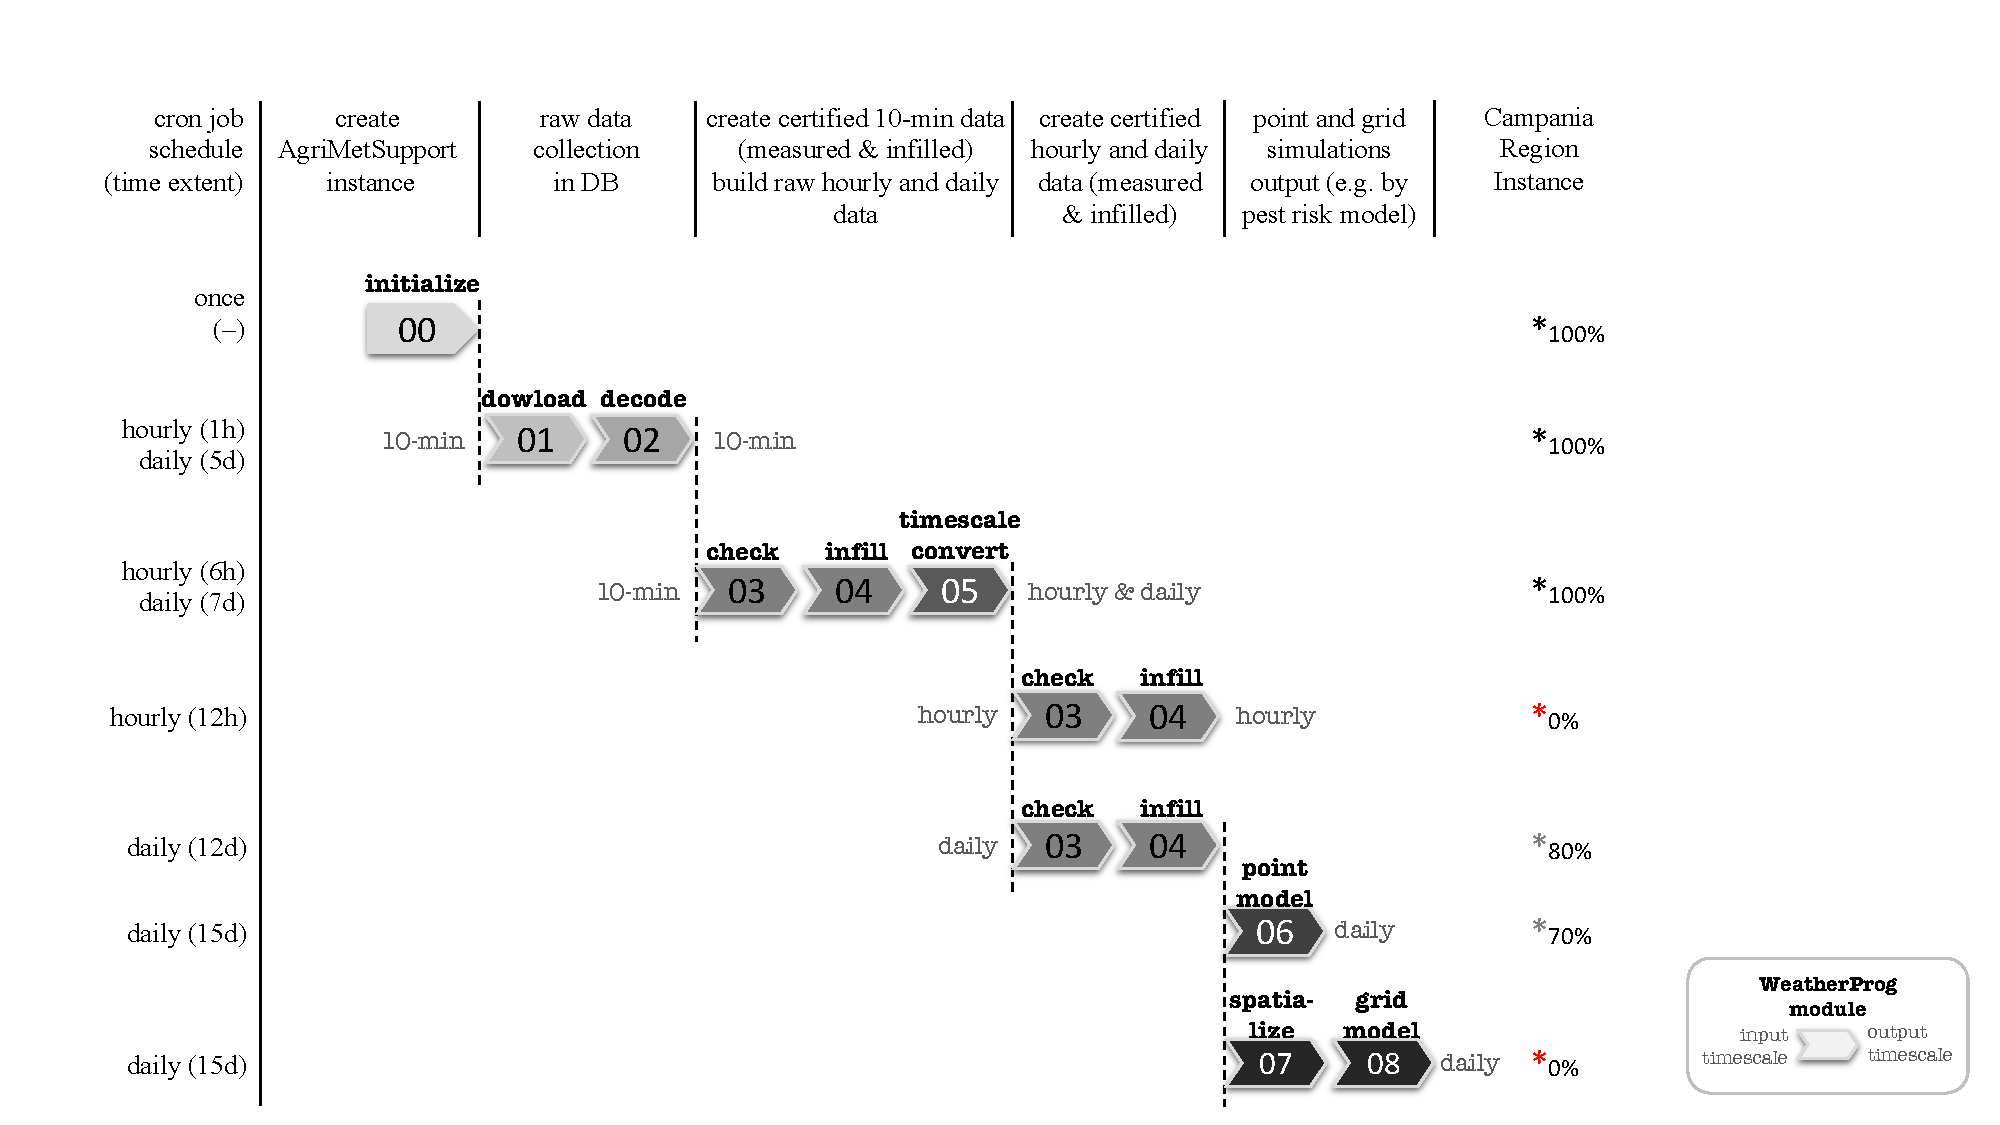
\includegraphics[scale=.4]{figures/WeatherProg_fig.pdf}
	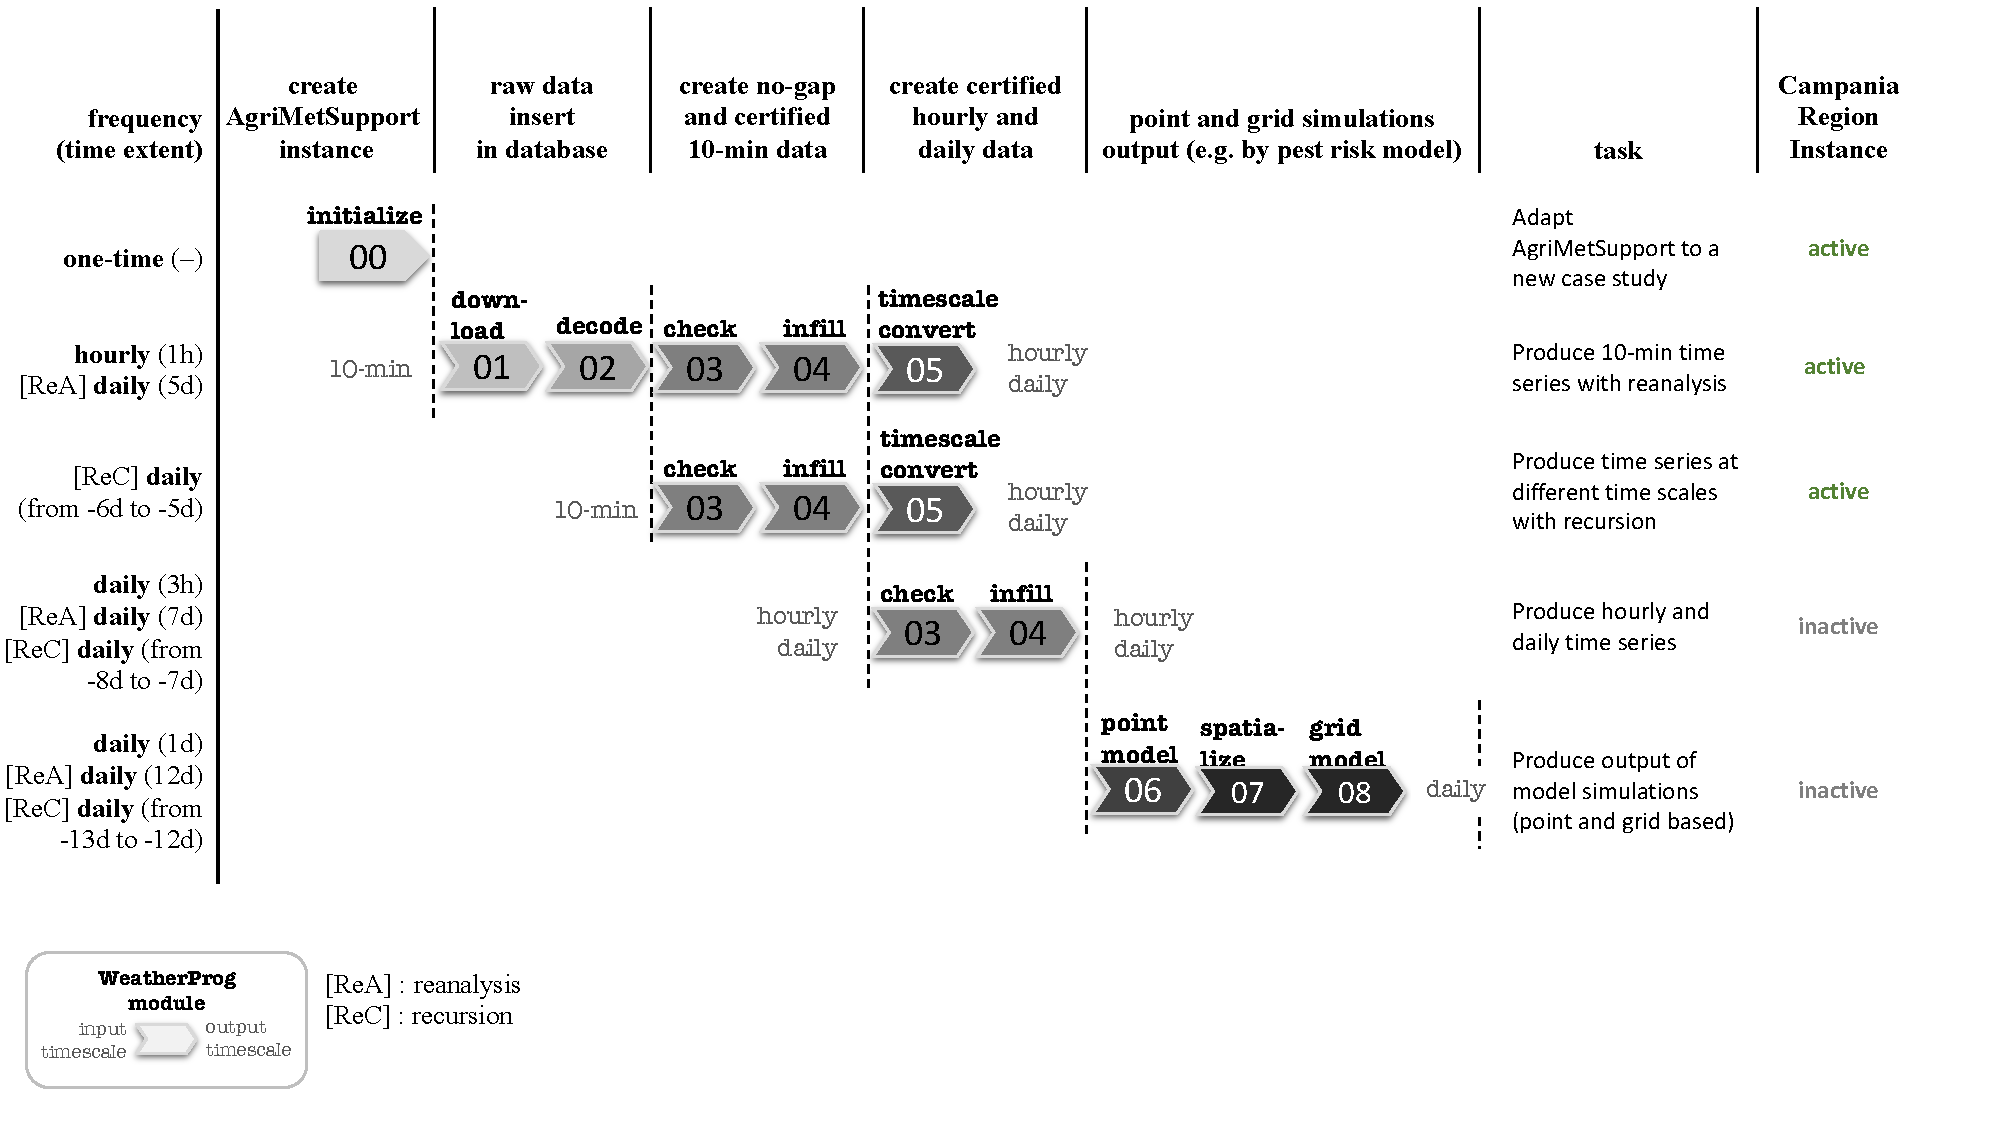
\includegraphics[scale=.4]{figures/WeatherProg-schedule-fig.pdf}
	\caption{WeatherProg cron job schedule for air temperature in a typical \gci instance. Each row of the schedule is a pipeline and pipelines are orchestrated to build homogeneous and complete agrometeorological database.}
	\label{Fig:weatherprog:calls}
\end{figure}


\section{Quality check procedure}[Giuliano][wip] \label{sec:qcheck}

\subsection{Quality check module (semi-automatic on demand)}
The quality check reads data stored in a relational database (in our case PostgreSQL)[UP]\\
and applies a procedure based on a multi-step and variable-oriented procedure.

NOTES: (flags and meaning: UP)\\
logic of the checks;\\
kind of checks (range, logic, climatologic, temporal, spatial, ...)

\begin{itemize}
    \item qcheck m10, T + R
    \item qcheck h1,  T + R
    \item qcheck h24, T + R
\end{itemize}


\paragraph{Control flags}\label{controlFlags} % TODO Polish control flags
Each of the flags for the quality control modules can assume one of the following values \note{[provided a Table]}:
\begin{table}[]
    \begin{scriptsize}
    \centering
    \begin{tabular}{r|p{10cm}}
    \multicolumn{2}{c}{Blablabla} \\
    \hline
	UNPROCESSED & The measurement has not been subject to the quality control yet\\
	DISABLED & The quality control module \note{(or the kind of quality check?)} was not enabled for this measurement\\
	UNCHECKED & Quality control was performed on this measurement, but this specific quality control \note{kind} has not been applied yet\\
	CORRECT & This measurement appears to be correct according to this quality control \note{kind} \\
	DUBIOUS & This measurement is suspicious, according to this quality control \note{kind}, which cannot decide either for correctness or for wrongness. A knowledge-based human checking is required \\
	UNDECIDED & The measurement has been subject to some quality control \note{kind}, but the procedures have not ended yet \note{GL: not clear to me!}\\
	WRONG & This measurement appears to be wrong according to this quality control \note{kind} \\
	%MISSING & This measurement is not present in the database \note{remove}\\
	%INVERTED & This measurement of a maximum (minimum) value of a climatic variable appears to be inverted with its respective minimum {maximum} \note{remove}\\
    \end{tabular}
    \caption{Flags used in the quality check module.}
    \label{tab:flagsSummary}
    \end{scriptsize}
\end{table}

\note{add a table to map flags with kinds of quality checks in order to get the overall flags, reported in the list below.}

On the other hand, for the overall quality control flag the following values are defined (see \cref{Fig:weatherprog:calls}).


\section{Case study: \gci at work in Campania Region}[Giuliano][wip] \label{sec:casestudy}

An \gci instance was tailored to the requirements of the Campania Region.
This is of particular relevance considering huge limitations and constraints therein present.
Important limitations are the eco-environmental complexity of the study area, the scarcity of stations and the lack of long term time series for any station.
Other constraints are the urgent need for monitoring and sharing agrometeorological data in the regional territory %(highlight the important step forward thanks to our GCI)
and the urgent need for a system to assist the production of bulletins to help mitigate the effects of alien or autochthonous pests.
 
\subsection{Study area}[Giuliano][done]
Located in southern Italy between \ang{13;45;}E, \ang{15;49;}E, \ang{39;59;}N and \ang{41;31;}N, Campania is the third most populated region of the Country, but due to its extension of about \SI{13600}{\metre\squared}, it is the most densely populated region of Italy.
Its inland is occupied by the Apennine Mountains, oriented roughly NW-SE, whereas the Sele and Campana plains border the coast.
The Sele plain is named after the river which traverse it, while the Campana plain is traversed by the Volturno river.
Nevertheless, the majority of the regional territory is hilly, for the 50\% of the territory, against the 35\% mountainous and the 15\% flat.
Consequently, the elevation ranges from \SIrange{0}{1904}{\metre} above mean sea level.

%     AGRONOMIC INFO e.g. the production of products of particular quality (DOP, IGP, DOC, DOCG; ...)
Since a large part of the territory is mountainous, the only agricultural zones exploited for cultivation are flat and partly hilly, even though a large pressure from urbanisation caused huge land take during the past decades, in particular  the coastal zones in Napoli, Salerno and Caserta, with cities having the highest population densities in whole Europe (i.e. Portici municipality).

Cultivated lands are favoured by the very fertile soils of volcanic origin and from the availability of water. 
Therefore, Campania is characterized by the high productivity of lands and by the high quality of agricultural products.
It holds a supremacy in Italy and abroad in the production of tomatos, potatoes, eggplants, peppers and peas, besides the fruit of fig trees, hazel trees, citrus fruit, apricots, plum, chestnut and cherries. 
Very important is also the production of wine and oil.
The breeding is constituted in good part from cattle and buffalos, characteristic of the region is the production of the famous buffalo's mozzarella, exported worldwide.

%    AGRO-ECONOMY\dots e.g. the ecomic value of the regional production in the primary sector

\subsection{Agrometereological network %in \gci instance
\label{RARStructure}}[Raffaele][done]

The WMO-compliant agrometereological monitoring network of the Campania Region comprises, at the time of this writing, only 34 stations, and this number is already insufficient to properly capture the complexity of the environment of the Campania Region.
To make things worse, the stations vary in their instrumentation, hence there is not any station which is capable of measuring all the 11 fundamental climatic variables, although each climatic parameter is measured by at least one station.
The bare minimum instrumentation includes sensors for air temperature, rainfall and air humidity, and 10 stations of the network measure only these three parameters.
The least monitored variable is air pressure, with only 9 stations currently measuring it.
\cref{tab:rarSummary} lists some statistics about the station network, while \cref{fig:rarLocations} illustrates the deployment of the stations over the territory of the Campania region.
\review{ Agrometeorologial stations are located from \SIrange{10}{770}{\metre} above mean sea level, highlighting scarce coverage of the complex regional territory. }

\begin{table}[]
    \centering
    \begin{tabular}{c|c|c}
        & \textbf{Active stations} & \textbf{All available data} \\ 
        \hline
        Number of stations & 34 & 38 \\
        \hline
        \multicolumn{3}{c}{General information} \\
        \hline
        Minimum elevation & \multicolumn{2}{c}{\SI{11}{\metre} a.m.s.l.}\\
        Maximum elevation & \multicolumn{2}{c}{\SI{769}{\metre} a.m.s.l.} \\
        Measurements time scale & \multicolumn{2}{c}{\SI{10}{\minute}} \\
        \hline
        \multicolumn{3}{c}{Lenght of the time series available in \gci} \\
        \hline
        1 year & 9 & 10 \\
        2 years & 23 & 26 \\
        3 years & 2 & 2 \\
        \hline
        \multicolumn{3}{c}{Stations per variable} \\
        \hline
        Air temperature & 34 & 38 \\
        Rainfall & 34 & 38\\
        Air humidity & 34 & 38\\
        Wind direction & 24 & 25\\
        Wind speed & 25 & 26\\
        Wind gusts & 25 & 26\\
        Air pressure & 9 & 10\\
        Solar radiation & 13 & 14\\
        Soil temperature & 13 & 13\\
        Soil humidity & 13 & 13\\
        Leaf wetness & 23 & 24 
    \end{tabular}
    \caption{Detail of the agrometereological network in Campania}
    \label{tab:rarSummary}
\end{table}

\begin{figure}
	\centering
	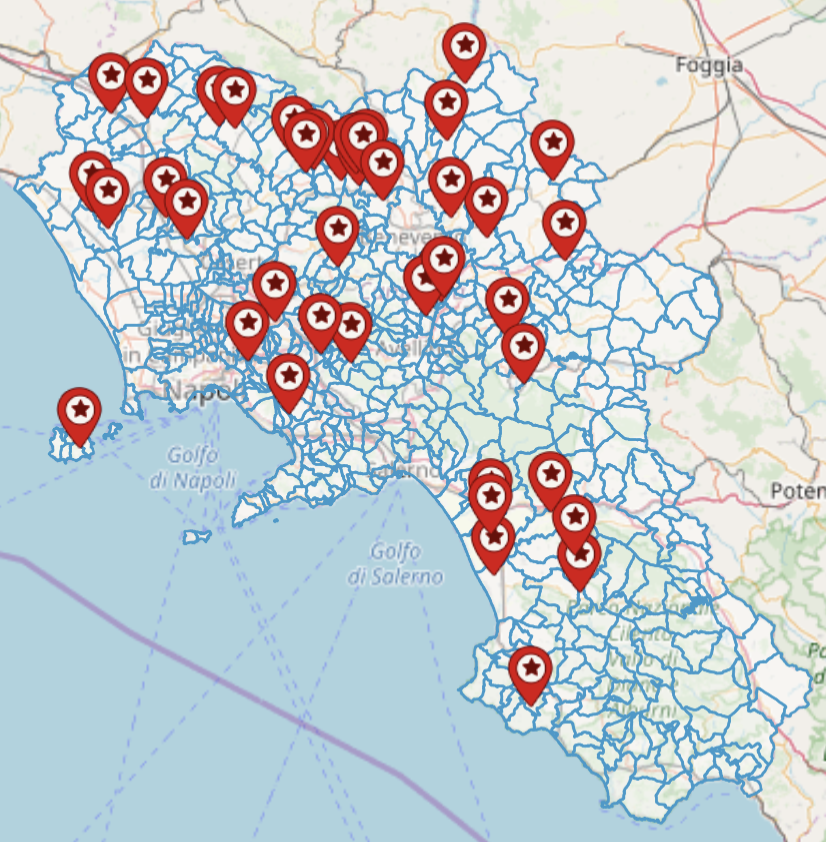
\includegraphics[scale=.8]{figures/rarLocations}
	\caption{ Geolocation of the stations included in the Regional database \review{(symbol * for stations inactive at the time of writing).)}}
	\label{fig:rarLocations}
\end{figure}

The monitoring network is in charge of the Agrometereological Regional Centre (CAR, \emph{Centro Agrometereologico Regionale}) under the Department for Agriculture of the Campania Region. The CAR is also in charge of producing pest risk bulletins for the agricultural farms of the Region.

\subsection{Retrieve and decode bulletin data}[Giuliano][done]
On hourly basis, the CAR send a bulletin containing the values of the measurements of the last 24 hours, on a 10-minute time scale. Each entry of the bulletin represents a point in time, and includes the values of all the variables measured by all the stations. The bulletin is sent via sFTP to a server located on the premises of the CRISP.
In order to recover for possibly late measurements, on daily basis a recap bulletin is sent, including all the measurements of the last month, on a 10-minute time scale, with the same format of the hourly bulletin.

Data as received from CAR is not suitable to be inserted into the data base. Each record of the incoming table contains all the measurements of all the climatic variables of all the stations in the RAR; such a record would clearly be poor effective and poor efficient, pointlessly grouping in a single record unrelated data; not to mention that such a record would violate WMO prescriptions about proper handling of climatic data \citep{wcdmp:cdms}.
 
 More importantly, the incoming table labels measurement of the same climatic variable with different names, making any attempt of data analysis impossible. To make things worse, the format of the incoming table is subject to change. The most relevant task of the decoding module is to map the different names of the same climatic variable to a standardised attribute, which is also employed by the database.
 
 For performance reasons, the data insertion is performed with a single SQL INSERT statement per climatic variable. This means that, given the all-or-nothing behaviour of SQL statements, each record to be inserted must be valid, otherwise the whole insertion will fail. It is therefore Weatherprog's responsibility to ensure that all the data submitted to the database can actually be inserted.
 
 To this end, the decoding module checks whether the data to be inserted is already present, since the insertion of a duplicate record would be rejected by the database. These checks have been optimised in order to avoid an excessive overhead due to database access: each database query is highly time consuming, fairly regardless of the complexity of the query. For this reason, it is highly impractical to check the presence of each value independently, on the contrary more complex queries, with the capability of validating a larger share of the data to be inserted, have been developed.
 
As said earlier, data is sent from CAR on an hourly basis, containing all the measurements of the previous 24 hours.
To handle the hourly dispatch and provide data to the end users as soon as they are available, the system is configured to automatically have a run of Weatherprog every hour, according to the schedule in \cref{Fig:weatherprog:calls}.
This hourly run is in charge of updating the database with the data related to the last hour.
Late updates of the incoming data are dealt with by a periodic run of the reanalysis pipeline, but on daily basis.
%This daily run works on the whole 24-hour incoming table, check which time ranges are missing within the database and fills them.


\subsection{Quality check and data consulting}[Giuliano][todo]
\note{[include Qcheck + webapp for agrometeo data consulting]}\\
\note{highlight the connection with the running schedule in \cref{Fig:weatherprog:calls} and show the results of qcheck }\\

\begin{itemize}
    \item our GCI can be adapted to a (regional) agrometeo monitoring network to produce qchecked point and grid data
    \item thanks to this, whatever service can be mounted on it, such as (search for REFs for each item):
    \begin{itemize}
        \item crop simulation (e.g. for biomass production)
        \item irrigation water management
        \item fertilisation management
        \item pest risk management (use of pesticides)
        \item rural land use planning
        \item zoning (crops management)
        \item land capability and land evaluation
        \item landslides
        \item civil protection (and alerts)
        \item forest modelling, simulation and planning
        \item 
    \end{itemize}
\end{itemize}

\note{ elsewhere: [1](allowing temporal/spatial stats queries and embedding CUDA codes (on the client-side GUI) for fast calculation); [2] (Then also WeatherProg itself has major CUDA developments in order to speedup crucial and time-consuming calculations such that of making spatial interpolation at any pixel of the study area).) }

\section{Discussion}[Giuliano][todo]

\note{[MOVE ELSEWHERE]} The need for tools that can enhance the climatic data distribution, improving environment/farm management; this implies that in Italy (and also find the EU regulation and apply the discourse to EU itself) PAN advises administrative units in charge of agrometeorological publication to provide climatic data but also pests bulletins (by using possibly mechanistic modelling) based on climatic data which are able to support decision making at the farm level, with the result of decreasing the amount of pesticides with the twofold effect of reducing costs and diminishing environmental impact of by-products.

\begin{itemize}
    \item Are the low-cost stations good enough for
    \begin{itemize}
        \item Subsequent applications
        \begin{itemize}
            \item Quality control
            \item Data reconstruction
            \item Biological applications
        \end{itemize}
        \item Data publication
        \begin{itemize}
            \item Is it needed to inform end-users of the difference between the two kinds of station of can it be omitted?
        \end{itemize}
    \end{itemize}
    \item Short time interval, and only one point, for evaluation
\end{itemize}

\section{Conclusions}[Giuliano][todo]
\note{[COPIED]}(**) The importance of tools like the GCI / WeatherProg engine that can provide a support for agencies constrained to adopt such technological advancements/improvements to raise the quality of the delivered support they can offer to farmers and stakeholders.

\note{[COPIED]} There is an evident gap between raw agrometeorological observations made by sensors in gauges in a monitoring network and the necessity to provide public access to data of good quality in the form of multipoint time series or of a temporal stack of digital maps.

\note{[COPIED]} WeatherProg is able to fill this gap and to simplify(stress this concept, i.e. that WeatherProg simplifies al operations!!!!) the implementation of services (that are mandatory!) necessary to support agriculture for todays threatens and to coadiuvate decision making in environmental management. It includes the state of the art of methods embedded in the main modules of the program.

%% The Appendices part is started with the command \appendix;
%% appendix sections are then done as normal sections
\appendix

\section{Monitoring with Low-Cost Station}[Raffaele][todo]
This station is made of low-cost and open-source components, \ldots IoT, \dots \note{[3-4 lines max]} The station can be employed to integrate and reinforce existing networks in order to improve the coverage of the territory, with a limited expense. They can be easily moved from a location to another, so as to be concentrated in particular areas for the time needed to characterise it, and then moved to a different area. This is particularly convenient to carry out joint monitoring (e.g. a  joint agroclimatic and pest monitoring) to tune specific models (e.g. a model simulating pest risks). This station can be used also by farmers located in the same territory where \gci is up, to locally monitor agroclimatic variables and get more accurate support (e.g. using models' predictions).

\section{Data base}[Giuliano and after Raffaele][wip]
\note{(Give a higher-level description, including the flags, consider a Table, add a description and action taken column.)}\\
\note{Here we have only the relational database, but we have mentioned earlier the raster data base. Should we mention that the latter has not yet developed or do we have something? (GL:) We cited the array data base before, in this paper we'll focus on quality check, not mapping yet (so no extended raster db description at now)}

To implement the relational climatic data base, the PostgreSQL Data Base Management System (DBMS) \citep{postgres:postgresql} has been chosen. PostgreSQL is the fastest relational DBMS, and is open-source; but the most relevant reason for its choice is its comprehensive support of spatial data. PostgreSQL features natively a number of geometric types and operators over them but, most importantly, it comes with an optional, open-source, extension named PostGIS  \citep{postgis:postgis} for full support of geographic data. This extension is a cornerstone in our plan for future improvement of the automated system.

\paragraph{Data model}
% TODO Update the data model if needed
\note{Version 3.0, assuming that the merging of the climatic data has been carried out. Update accordingly otherwise}

The data model of the data base has been studied to help maintaining data consistency. Its design allows to avoid a number of unconsistencies thanks to the relational checks performed by the DBMS. 

The data model is illustrated in  \cref{ERD}, which illustrate the logic-level \emph{Entity-Relationship Diagram} (ERD), ready to be implemented in SQL automatically by means of the \emph{pgModeler} \citep{silva:pgmodeler} open source software. For the reader unfamiliar with data modeling, the boxes representing tables of the database, with the fields listed within each box. The diamond-marked links represent a reference from a table to another subject to \emph{referential integrity constraints}, which are validity checks automatically performed by the DBMS. Further details of the model are described in the caption of \cref{ERD}.

Each measurement site is represented by an entry of the \texttt{Station} table. A station is uniquely identified by its coordinates. The toponym field is indispensable since it is employed, along with the station's elevation, by the web application to label the station itself. The date when the station was added to the network is recorded, as well as the withdrawal date for these stations which have been dismantled. The Network field provides support for the integration of different monitoring network, which is discussed in all its aspects in \cref{Integration}.

Additional pieces of information which may be available for the station are stored in separate tables. The advantage of this choice is twofold. Firstly, due to the fact that records are physically stored sequentially in the mass memory,  it is faster to access shorter records rather than having to "jump" unnecessary, often empty fields. Lastly, with this design there is no space allocated in the quite common case that these pieces of information are not available, contrarily to the need to waste space for empty columns. This splitting is profitable since data in the separate tables are not needed by the day-to-day operations of Weatherprog, and are only seldom used by the web application.

The table \texttt{Station Addresses} stores additional information about the location, most notably the farm whether the station is hosted. In fact, this data is more meaningful for the low-cost stations, and it is often not available for the permanent station. The table \texttt{Device} holds additional information about the rig which actually performs the measurements. Currently, only the model of the device is available.

The other fundamental table is the \texttt{Measurements} table. The measurements of all the climatic variables of all the stations are stored in this table. This choice has been made to allow coalescing of accesses, since it has been observed that it is faster to execute a single complex query rather than several simpler queries. More specifically, the controls required by the decoding module can be performed on all the variables simultaneously, and the insertion of new data can be performed with a single SQL statement. Each measurement is uniquely identified by the station which performed it, the climatic variable measured and the date and time of the measurement, and is accompanied by a series of flags, one for each control module, as described in \cref{controlFlags}. It is worth mentioning that, due to the choice of not to have a weird identifier of the stations, the coordinates of the station end up in the \texttt{Measurements} table. The availability of this piece of data allows for avoiding SQL JOINS to perform spatially-parameterized queries on the measurements. Constraints are defined to avoid any "structurally" invalid data.

The \texttt{Equipment} table lists all the climatic variables each station can measure. The fact that is this the referring table of the referential integrity constraint from the \texttt{Measurement} table ensure that a measurement for a variable that a station is not able to measure \textbf{cannot be inserted}, and this is verified directly by the DBMS.

\begin{figure}
	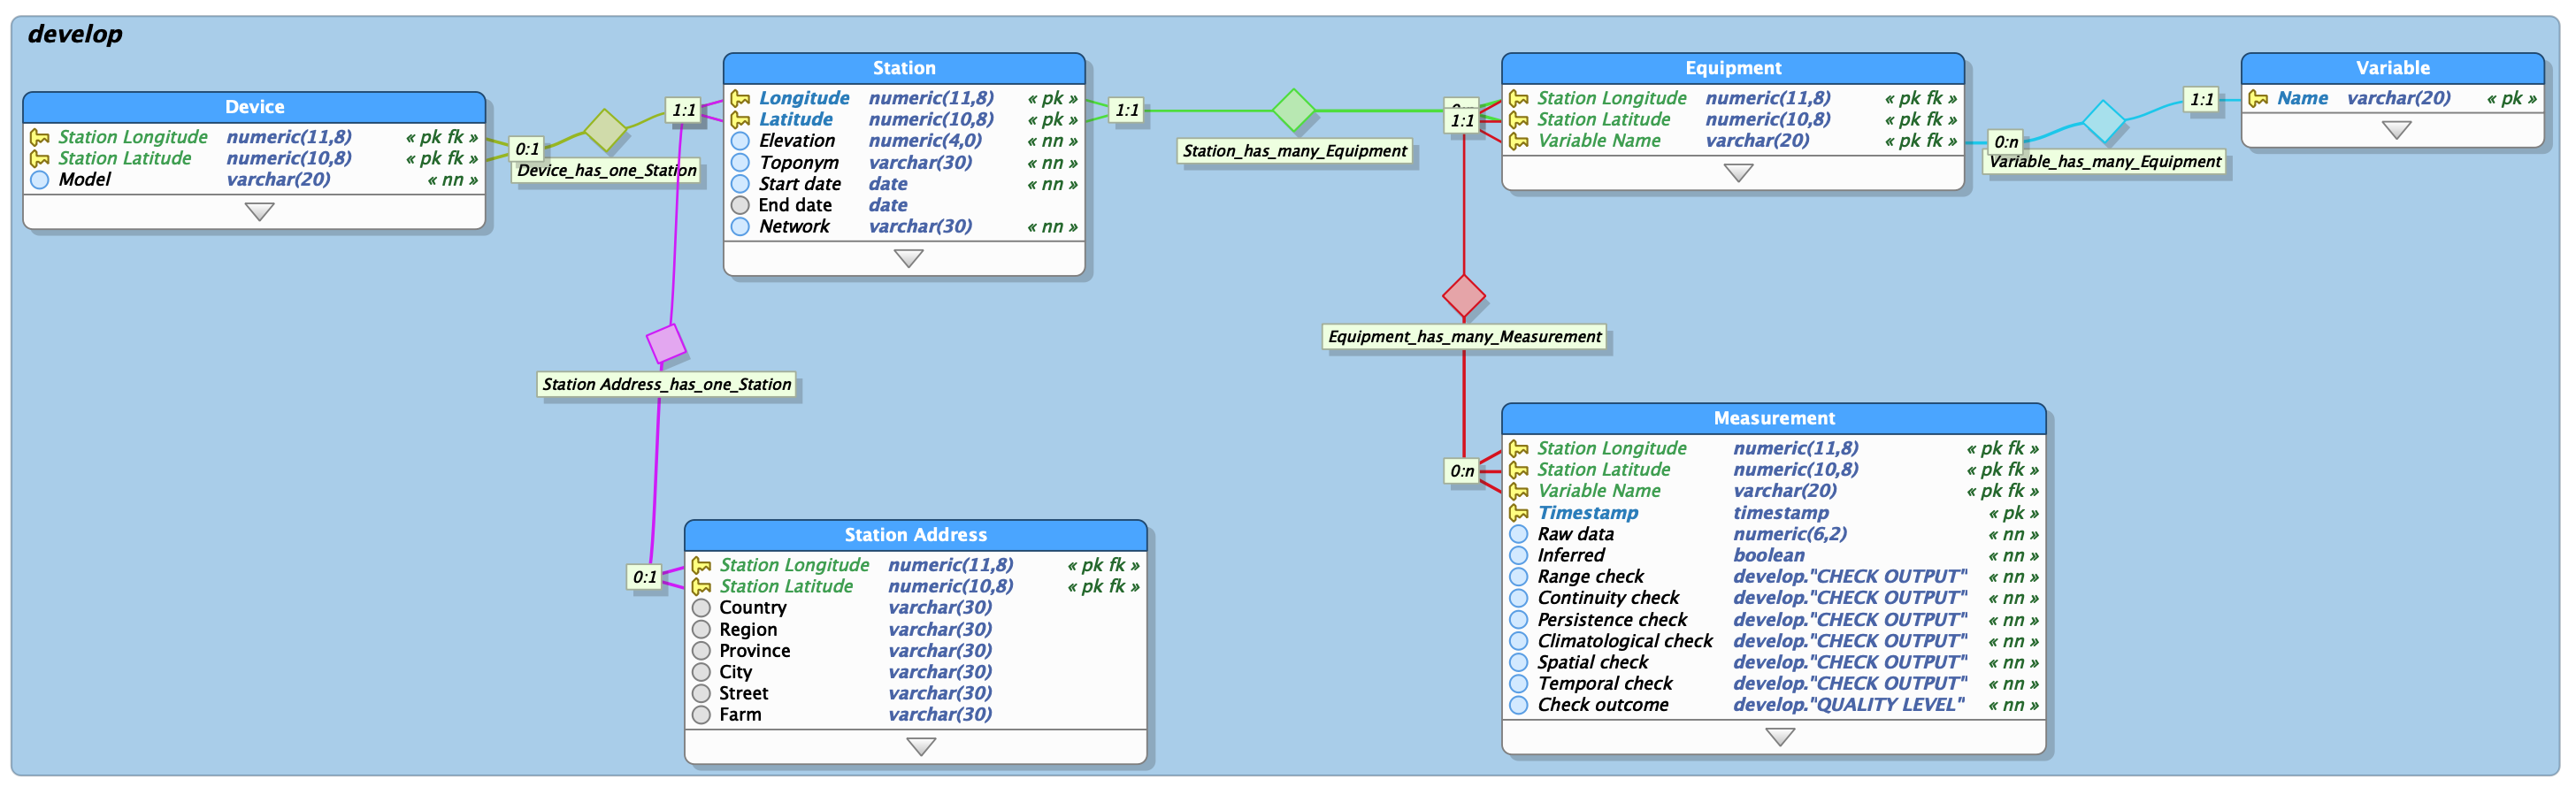
\includegraphics[scale=.26]{ERD}
	\caption{ \note{(move to tech full paper)} The data model for the climatic database. Each box represents a table. Each row in the box represents a field of the table. The yellow key denotes fields which form the Primary Key of the table. The blue circle denotes field which cannot be left empty by any record. Diamond-marked links means relationship within table subject to referential integrity constraints. Fields which are part of the Primary Key and subject to referential integrity constraints are written in green.\note{[enhance figure (do it again in powerpoint)]}}
	\label{ERD}
\end{figure}

\paragraph{Interface to WeatherProg}
Theoretically, Weatherprog could directly access the PostgreSQL database, by embedding SQL queries into the code of its core modules. This approach would strictly couple Weatherprog with the database structure, with the considerable downside of requiring to modify each and every relevant query in the code when a change of the database structure is applied. To enhance modifiability, we chose to have a dedicated persistence module instead. This way, Weatherprog's core modules no longer need to know, and therefore depend upon, every detail of the database architecture, instead it makes meaningful calls to the functions made available by the persistence module. Technically speaking, the persistence module, which is developed taking advantage of the object-oriented features of the Matlab\textsuperscript{\circledR} language, effectively provides an \emph{Application Programming Interface} (API) for using by the other modules of Weatherprog. When a structural change is applied to the database, the modification to the Weatherprog code is concentrated and limited to the persistence module, without affecting the other modules.

\subsection{The dashboards}[Raffaele][todo]
\note{May well be merged into the general description, unless we want to be very detailed in the description of what we have}\\
agrometeo data consulting (hopefully version 3.0 with QCheck!)\\
agrometeo network manager (we have something\ldots) \note{[read the overleaf comment and discuss about this opportunity]}\\
pest service consulting (we have the demo Plasmopara!!!)\note{[yes, but maybe it's better to move this piece to another paper, where pest models are in place (e.g. the LCN paper!)]}\\

\section{\note{[MOVE TO LCN]} Integration of the monitoring networks\label{Integration}}[Giuliano][done]
In this paragraph we describe the existence of more monitoring networks having different characteristics in the same study area.
This means that a higher degree of generality in the logic of the qcheck framework is required.
For this purpose, we tested the qcheck to both the permanent and low-cost network
\begin{itemize}
    \item Per-variable comparison between permanent and low-cost stations co-located at Pignataro Maggiore
    \item Evaluate "scostamento" in raw data between LC and P stations (all variables) to assess performance of the LC station
    \item After quality control (temperature, rainfall)
    \begin{itemize}
        \item Re-evaluate difference LC-P to re-assess performance after quality control and data reconstruction 
        \item Evaluate effect of LC stations error
        \begin{itemize}
            \item Pure thermal accumulation
            \item Biological application
        \end{itemize}
    \end{itemize}
\end{itemize}

%% \section{}
%% \label{}

%% If you have bibdatabase file and want bibtex to generate the
%% bibitems, please use
%%
  \bibliographystyle{elsarticle-harv} 
  \bibliography{biblio-items.bib}

%% else use the following coding to input the bibitems directly in the
%% TeX file.

%% \begin{thebibliography}{00}

%% \bibitem[Author(year)]{label}
%% Text of bibliographic item

%% \end{thebibliography}

\subsection{Monitoring with Low-Cost Stations}[Giuliano][todo]
\note{include in the same map both networks if possible and develop few text description}\\
The particular installation performed at 4 (or more) locations\ldots



\end{document}

\endinput
%%
%% End of file `elsarticle-template-harv.tex'.
